\documentclass[11pt]{article}
\usepackage[margin=1in]{geometry}
\usepackage{graphicx}
\usepackage{booktabs}
\usepackage{array}
\usepackage{tabularx}
\usepackage{longtable}
\usepackage{float}
\usepackage{hyperref}
\hypersetup{colorlinks=true, linkcolor=blue, urlcolor=blue}
\setlength{\parindent}{0pt}
\setlength{\parskip}{0.6em}
\begin{document}

{\Large \textbf{LiveCodeBench repaired RFM stage report}}\\
Generated: 2026-04-21 19:51 UTC

\section*{Object}
This report freezes the current \textbf{LiveCodeBench-only} stage on the same prompt-level label family used by the other probe surfaces: \texttt{majority\_s\_0.5}, defined here as a prompt being positive when a strict majority of its four saved rollouts have relative length greater than \texttt{0.5}. The saved March archive still carries an archive-time tail bit at \texttt{0.9}, so the stage label is recomputed from saved rollout lengths rather than read from the archive bit directly.

The frozen source train pool has 640 prompts. The detector fit-train split uses the same stage-materialization contract as the other probe lanes, including \texttt{balance\_train=downsample}, which yields 280 fit-train prompts, 128 validation prompts, and 160 test prompts. Positive counts are 140, 35, and 54 respectively.

\begin{table}[H]
\centering
\begin{tabular}{lrr}
\toprule
Split & Prompt count & Positive count \\
\midrule
Source train pool & 640 & -- \\
Fit-train & 280 & 140 \\
Validation & 128 & 35 \\
Test & 160 & 54 \\
\bottomrule
\end{tabular}
\caption{LiveCodeBench repaired prompt object.}
\end{table}

\section*{Detector comparison}
The selected RFM detector row is layer 27 with bandwidth 100, validation PR-AUC 0.6555, and test PR-AUC / ROC-AUC 0.7055 / 0.8590. This is a real improvement over the prompt-only and activation-linear baselines on the repaired object, but it is not a clean activation-MLP win: activation MLP last-layer under the \emph{best-rank} checkpoint rule is essentially tied on PR-AUC, and under \emph{best-loss} it is slightly higher.

\begin{figure}[H]
\centering
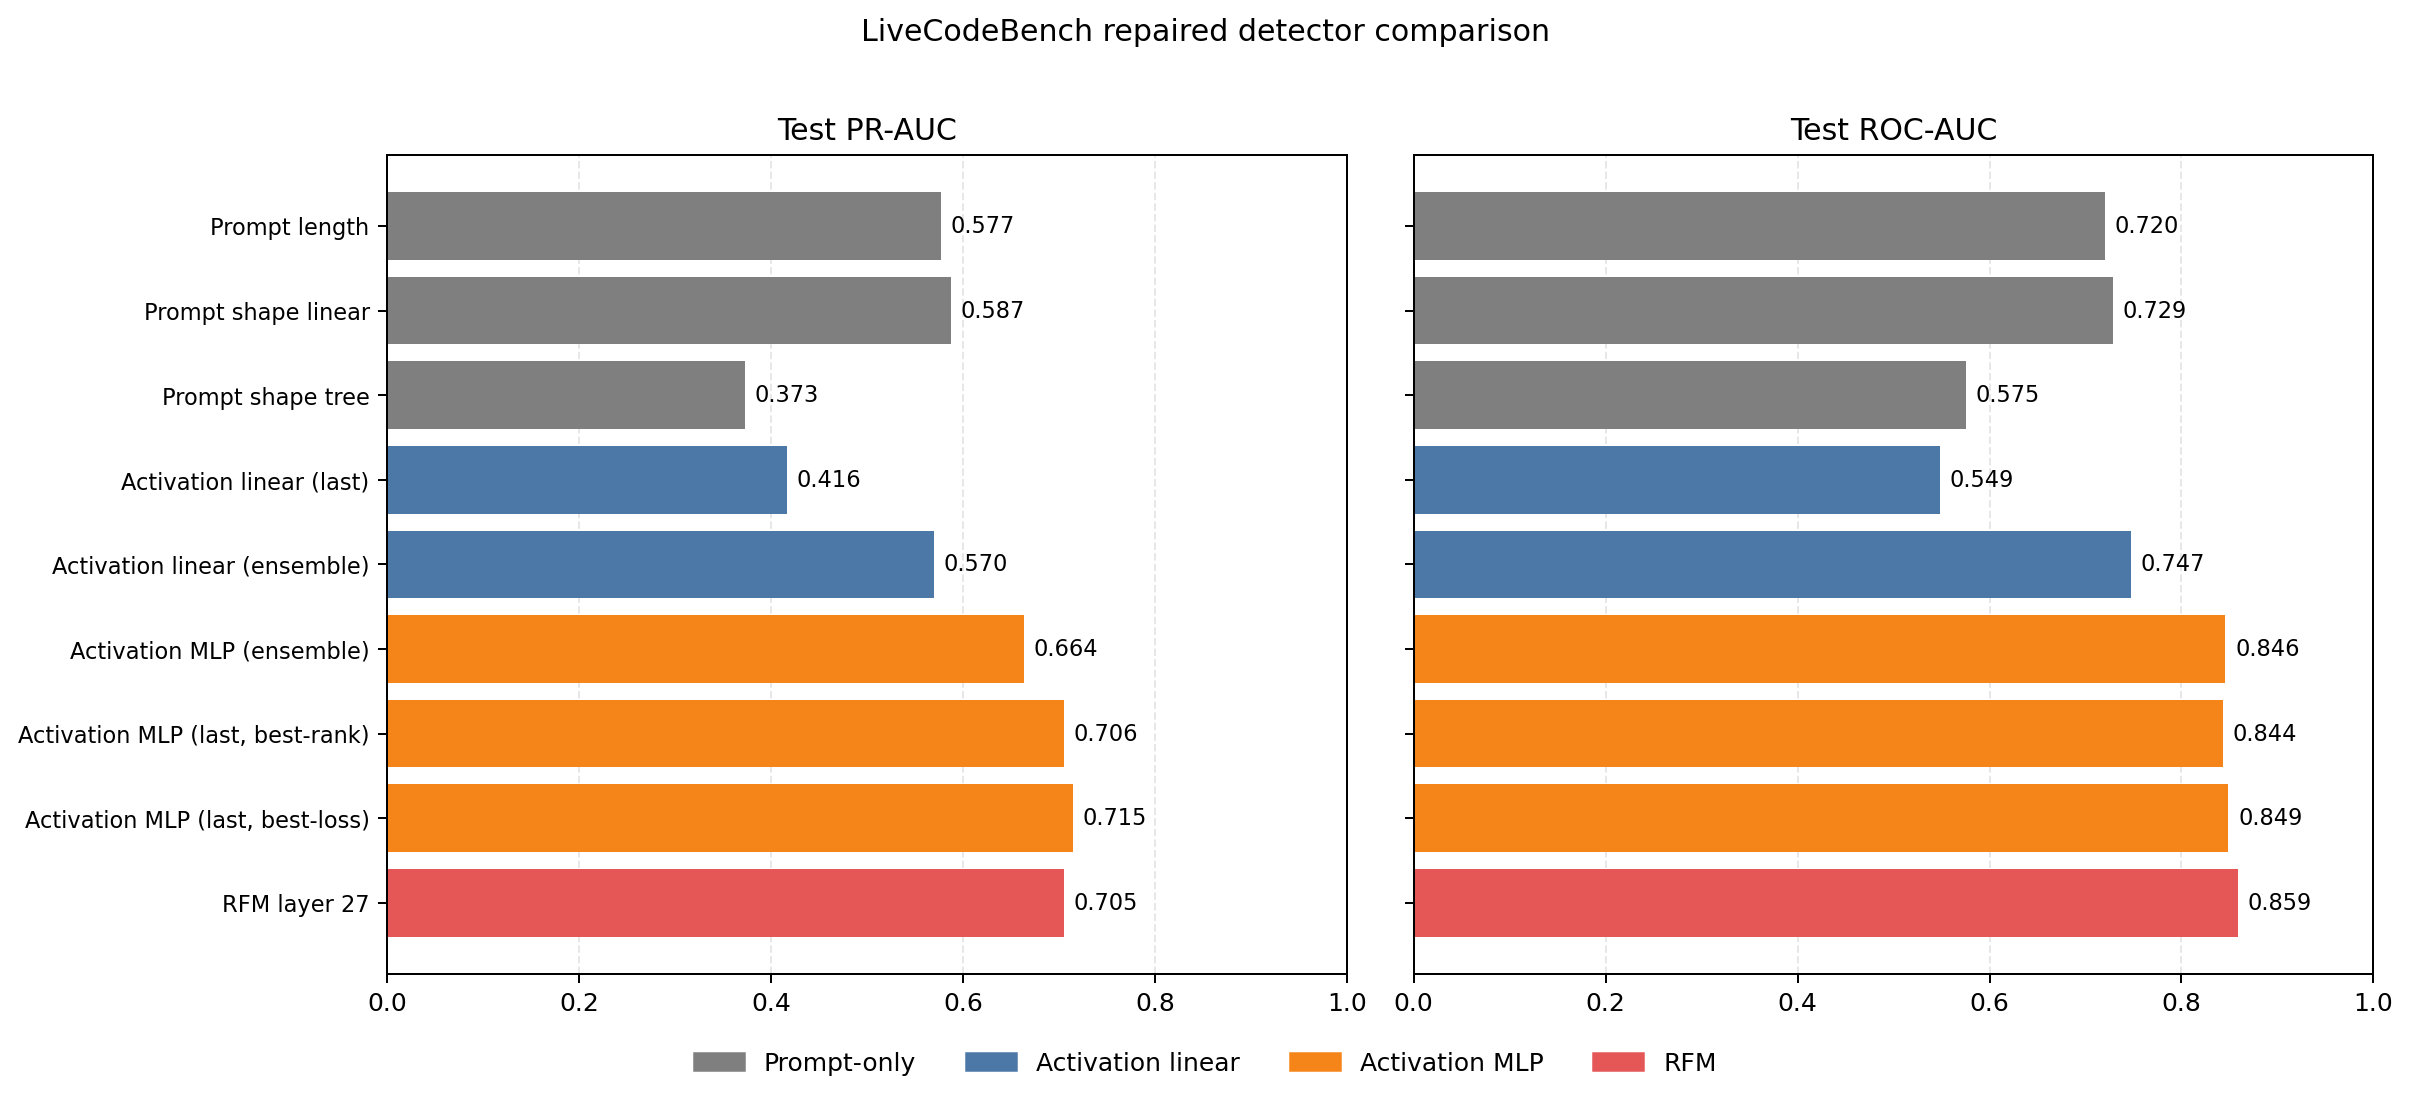
\includegraphics[width=0.98\textwidth]{detector_comparison.png}
\caption{Test-set detector comparison on the repaired LiveCodeBench object. Prompt-only rows are single-model fits; activation rows are three-seed means; RFM is the selected single-seed layerwise detector.}
\end{figure}

\begin{table}[H]
\centering
\begin{tabularx}{\textwidth}{>{\raggedright\arraybackslash}p{0.39\textwidth}>{\raggedright\arraybackslash}p{0.25\textwidth}rr}
\toprule
Method & Group & Test PR-AUC & Test ROC-AUC \\
\midrule
Prompt length & Prompt-only & 0.577 & 0.720 \\
Prompt shape linear & Prompt-only & 0.587 & 0.729 \\
Prompt shape tree & Prompt-only & 0.373 & 0.575 \\
Activation linear (last) & Activation linear & 0.416 & 0.549 \\
Activation linear (ensemble) & Activation linear & 0.570 & 0.747 \\
Activation MLP (ensemble) & Activation MLP & 0.664 & 0.846 \\
Activation MLP (last, best-rank) & Activation MLP & 0.706 & 0.844 \\
Activation MLP (last, best-loss) & Activation MLP & 0.715 & 0.849 \\
RFM layer 27 & RFM & 0.705 & 0.859 \\
\bottomrule
\end{tabularx}
\caption{Exact metrics used in the detector plot.}
\end{table}

\section*{Direction quality}
The stage-2 object is no longer hypothetical. The exported vector bundle carries 100 bootstrap replay fits per layer under the fixed selected hyperparameters. All 28 layers have mean cosine at least 0.781 to the exported signed direction; the weakest 95\% lower bound across layers is 0.693. The most stable layers are 26 (0.909), 25 (0.901), 14 (0.896), 8 (0.891). The selected detector layer 27 is stable enough to be usable but is not the most coherent layer: its mean cosine is 0.786 with lower bound 0.734. Its 1D projection score also remains predictive on held-out data (test PR-AUC 0.7150).

\begin{figure}[H]
\centering
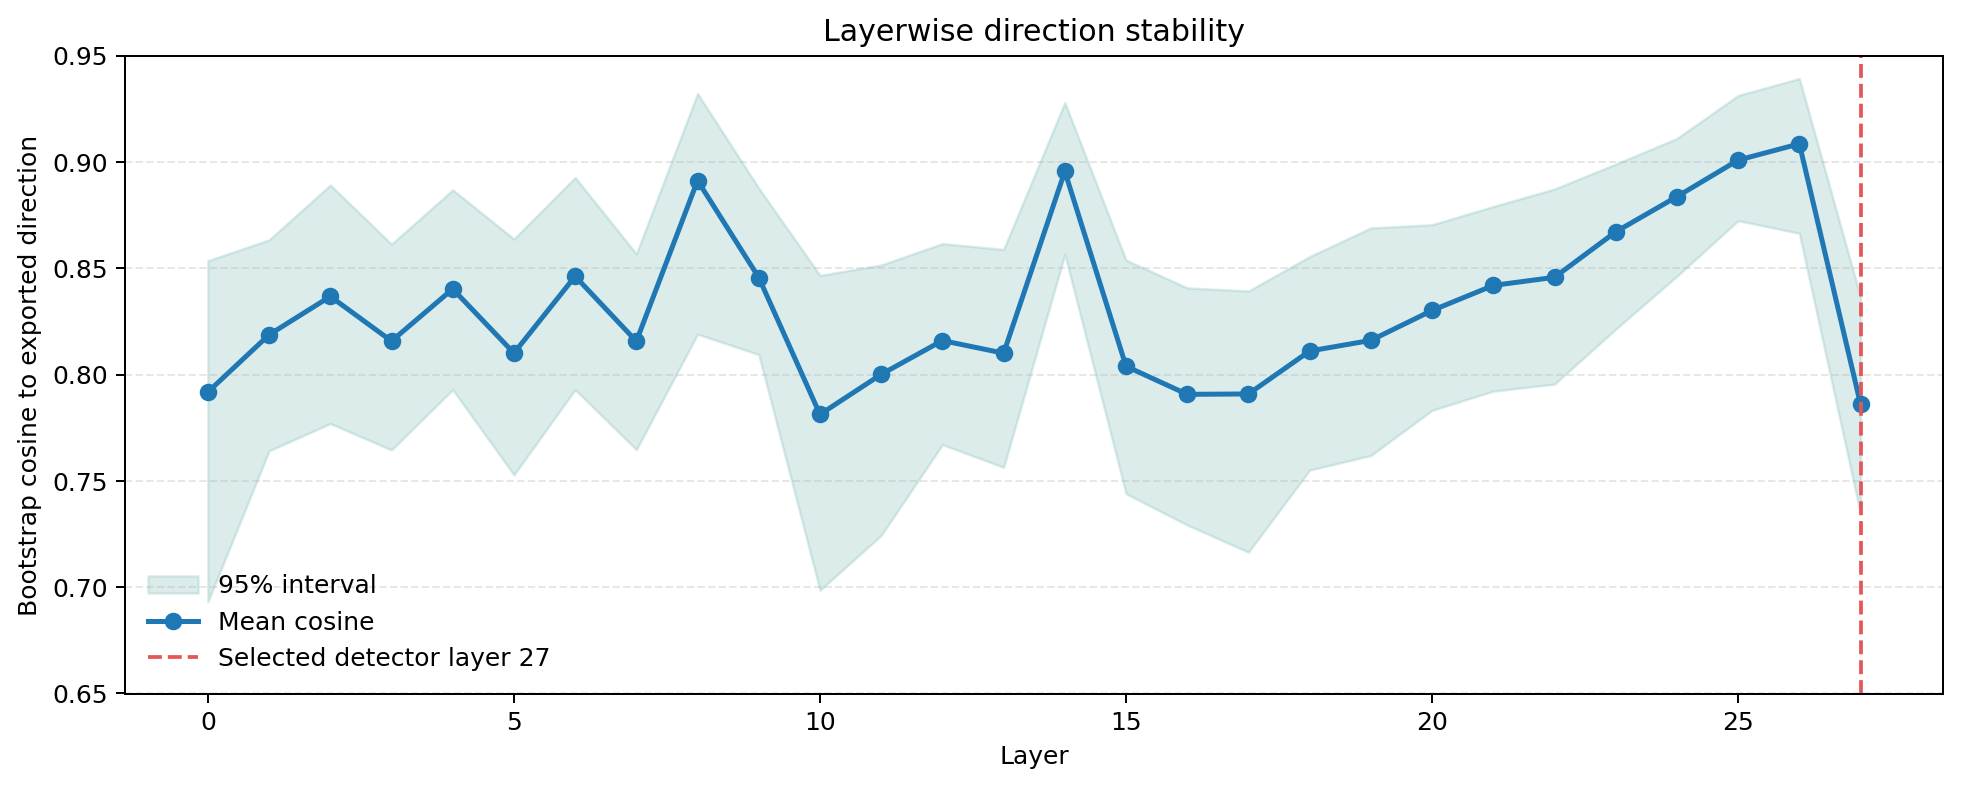
\includegraphics[width=0.92\textwidth]{direction_stability.png}
\caption{Bootstrap cosine stability for the exported per-layer LiveCodeBench directions.}
\end{figure}

\section*{Benchmark-local spherical steering}
The first larger repaired control table is now complete on 32 held-out LiveCodeBench prompts with fixed spherical strength \texttt{t = 0.3} at the hook site \texttt{prefill\_layer\_output\_last\_token}. All four conditions stay at 0/32 \texttt{pass@1}. The loop-fraction read is negative rather than merely inconclusive: baseline \texttt{no\_steer} is 0.03125, while \texttt{minus\_v\_spherical} is 0.28125, \texttt{plus\_v\_spherical} is 0.125, and \texttt{random\_spherical} is 0.34375.

\begin{figure}[H]
\centering
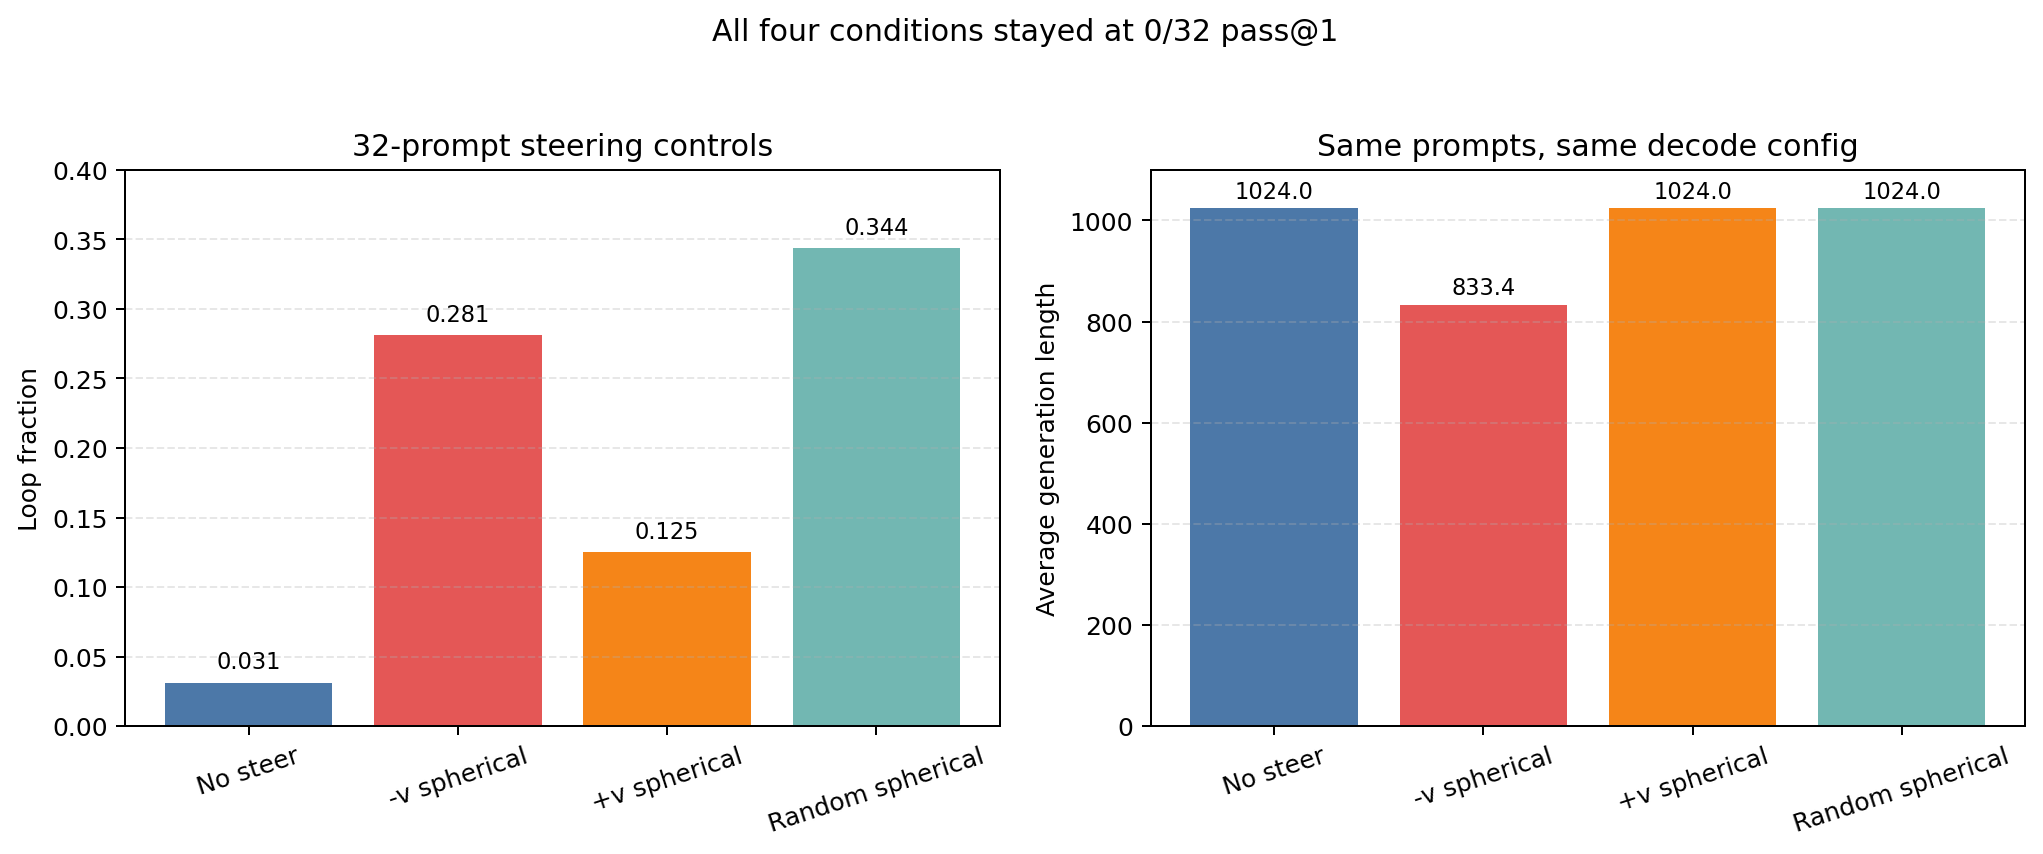
\includegraphics[width=0.98\textwidth]{steering_controls.png}
\caption{Finished 32-prompt spherical steering controls. All conditions stay at 0/32 pass@1, and every steered arm is worse than baseline on loop fraction.}
\end{figure}

\section*{Provenance}
Detector training commit: \texttt{120a808bf0ed}. The steering table was generated from commit \texttt{26a94687531b} with vector bundle hash \texttt{46422ae875f7}. The grader version is \texttt{livecodebench\_codegen.re}.

The full machine-readable bundle for this report includes exact prompt IDs, prompt-ID hashes, vector checksums, per-condition artifact hashes, and the copied source receipts in \texttt{source\_data/} alongside \texttt{livecodebench\_stage\_summary.json}.

\section*{Bottom line}
The LiveCodeBench repaired stage is finally concrete enough to hand over as a report rather than a thread summary. The honest read is:
\begin{itemize}
\item detector side: RFM is real and competitive, but not a clean activation-MLP win;
\item direction side: the exported bundle is stable enough to study causally;
\item steering side: the current benchmark-local spherical protocol is negative on the first larger held-out table.
\end{itemize}

That means ``finish LiveCodeBench'' at this stage does \emph{not} mean ``claim steering works.'' It means the repaired LiveCodeBench object, detector comparison, vector-quality read, and first benchmark-local steering control table are now all frozen into one deliverable surface.

\end{document}
